%%%%%%%%%%%%%%%%%%%%%
% 4章
%%%%%%%%%%%%%%%%%%%%%
\chapter{ヒューリスティクスを用いた手法} \label{chapter:4}

本章では,選挙区割問題を解くヒューリスティクスを作り,
その解から得られた選挙区の人口上限と下限を用いて,
ZDD構築を効率化する手法について提案する.

\section{概要}

\ref{chapter:3}章の人口制約付きZDD構築アルゴリズムでは,
パラメータとして部分グラフの重み上限$U$,下限$L$を用いた.
許容格差定数$r$を用いると,$r$の値によって,
$U, L$の範囲が必要以上に広くなることや
$U, L$の範囲に解が一つも存在しないことがあり得る.
既存手法では,$r$の値を都道府県によって手動で調整するものがほとんどである.
そこで,本研究は選挙区割問題をヒューリスティクスで解き,
解として得られる選挙区から,
最大人口の選挙区の重みを$U$,最小人口の選挙区の重みを$L$
と定義する手法を提案する.
$U, L$が最適解に近くなればなるほど,ZDDの構築時に,
最適解でない解候補の枝刈りの回数が多くなる.
その結果,従来手法に比べて
メモリの使用量の減少及び計算時間の短縮が期待できる.

\begin{figure}[htbp]
  \centering
  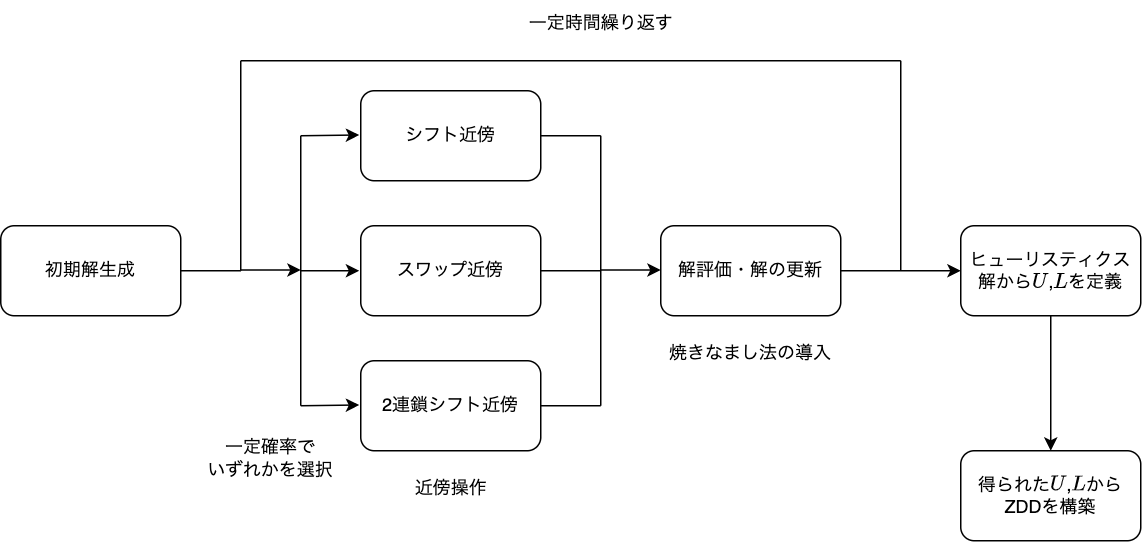
\includegraphics[scale=0.39]{img/heuristics.png}
  \caption{ヒューリスティクスを用いた提案手法}
  \label{heuristics}
\end{figure}

ヒューリスティクスでは,解を$x$とおき,
評価に用いるスコアを,$f(x)=\frac{\mathrm{max}(P)}{\mathrm{min}(P)}$として,
これを最小化することを目指す.

提案手法の全体像を図\ref{heuristics}に示す.
始めに選挙区割問題の初期解を生成し,次に一定の確率で
シフト近傍,スワップ近傍,2連鎖シフト近傍のいずれかを選択する.
選択した近傍操作を行って近傍解を生成し,
近傍解が選挙区割の制約(選挙区が$d$個のみ存在する,飛び地がない)を満たすか判定をする.
制約を満たしている場合には,スコアを計算し,
焼きなまし法により解の遷移を行う.
これを一定時間繰り返すことで,解を得ることができる.
その解から,$U = \mathrm{max}(P), L = \mathrm{min}(P)$
を定義し,それらを用いてZDDを構築する.
次節から,初期解生成や近傍探索のアルゴリズムについて詳細に説明する.

\section{初期解生成} \label{section:4.2}

初期解は,市区町村を表現したグラフから
選挙区を構成する部分グラフの$d$個の根を定め,
それぞれの根から幅優先探索(BFS)を行い,探索した頂点を
部分グラフに含めることで構築する.
初期解生成の擬似コードを\textbf{Algorithm 4}に示す.

\begin{breakablealgorithm}
  \caption{MakeInitialSolution}
  \label{make_initial_solution}
  \begin{algorithmic}[1]
    \Require $n, d, ave, adj\_list, w$
    \Ensure $x$
    \State $x \gets [-1] * n$
    \State $P \gets [0] * d$
    \State 頂点重みが最も大きいものから順に$d$個の頂点番号を配列$root$に保存する.
    \State $root$.reverse()
    \For {$i = 1,\ldots,d$}
      \State $queue \gets \phi $
      \State $x[root[i]] \gets i$
      \State $P[i] \gets P[i] + w[nv]$
      \State $queue$.enqueue$(root[i])$
      \While{$queue$.size() $\neq 0$ and $P[i] < ave$}
        \State $v \gets queue$.dequeue()
        \ForAll {$nv \in adj\_list[v]$}
          \If {$P[i] \geq ave$}
            \State break
          \ElsIf {$x[nv] = -1$}
            \State $x[nv] \gets i$
            \State $P[i] \gets P[i] + w[nv]$
            \State $queue$.enqueue($nv$)
          \EndIf
        \EndFor
      \EndWhile
    \EndFor
    \While{$x$の要素に$-1$が含まれる}
      \For {$vi = 1,\ldots,n$}
        \If{$x[vi]=-1$}
          \ForAll {$nv \in adj\_list[v]$}
            \If{$x[nv] \neq -1$}
              \State $x[vi] \gets x[nv]$
              \State break
            \EndIf
          \EndFor
        \EndIf
      \EndFor
    \EndWhile
    \State \textbf{return }$x$
  \end{algorithmic}
\end{breakablealgorithm}

\textbf{Algorithm 4} MakeInitialSolution の入力と出力については以下の通りである.\\
\textbf{入力}
\begin{itemize}
  \item $n$:グラフの頂点$v$の個数
  \item $d$:区割(グラフ分割)数
  \item $ave$:一選挙区の平均人口
  \item $adj\_list$:グラフの隣接リスト
  \item $w$:グラフの頂点重み
\end{itemize}
\textbf{出力}
\begin{itemize}
  \item $x$:頂点番号を添字とした配列で,
    選挙区(部分グラフ)のラベル(値は$1,\ldots,d$)が保存されている.初期値は$-1$.
\end{itemize}

2行目の$P$は部分グラフごとの重み和を保存する変数である.
配列$root$は,BFSの始点となる$d$個の頂点を含める.
3行目にもある通り,$root$は頂点重みが最も大きいものから順に指定する.
4行目で$root$を逆順にするが,これは$root$の頂点重みが小さいものから
探索を行うためである.
BFSでは,キューを用いて探索を行い,
探索した頂点を属する部分グラフに加えていく(5-22行目).
ラベル$i$の探索では,頂点$nv$を追加する際に
$x[nv]$に$i$を代入し,部分グラフの重み和$P[i]$に
$w[nv]$を加算する.
そして,重み和$P[i]$が平均重み$ave$以上になると,
その部分グラフでの探索を中断する(10,13行目).
これを全ての根$root[1],\ldots,root[d]$に対して行う.
全てのBFSを終えた後,ラベルが付かなかった($x$の値が$-1$の)
頂点に対して隣接頂点を参照し,そこからラベルを割り振る
処理を行なっている(23-34行目).
最後に$x$を出力し,これを初期解とする.

\section{近傍操作}

近傍操作とは,現在の解から少し形を変えた近傍解を生成する操作のことである.
選挙区割問題における近傍操作では,次の3つを定義する.
\begin{itemize}
  \item シフト近傍
  \item スワップ近傍
  \item 2連鎖シフト近傍
\end{itemize}

3つの近傍操作は確率を用いてその都度ランダムに選択する.
近傍解は,問題の制約を満たさない
(部分グラフが$d$個存在しない,連結でない)
場合があるため,その都度BFSなどを用いて判定を行う.
近傍解が問題の制約を満たしている場合,
焼きなまし法の手順に沿って解を改善していく.

\subsection{シフト近傍}

シフト近傍は,1頂点のラベルを変更する近傍操作である.
シフト近傍の例として,図\ref{shift-neighbor}を用いて説明する.
青色の頂点集合からなる部分グラフを$\mathcal{G}_1$,
赤色の頂点集合からなる部分グラフを$\mathcal{G}_2$とする.
$\mathcal{G}_1$には頂点$v_1$が含まれており,$v_1$は,
別の部分グラフ($\mathcal{G}_2$)の頂点$v_2$と隣接している.
シフト近傍では,頂点$v_1$のラベル$x[v_1]$を
頂点$v_2$のラベル$x[v_2]$に代入することで,
$v_2$を$\mathcal{G}_2$から$\mathcal{G}_1$に含めることができる.
こうしてできた新たな解$x$を近傍解とする.

\begin{figure}[htbp]
  \centering
  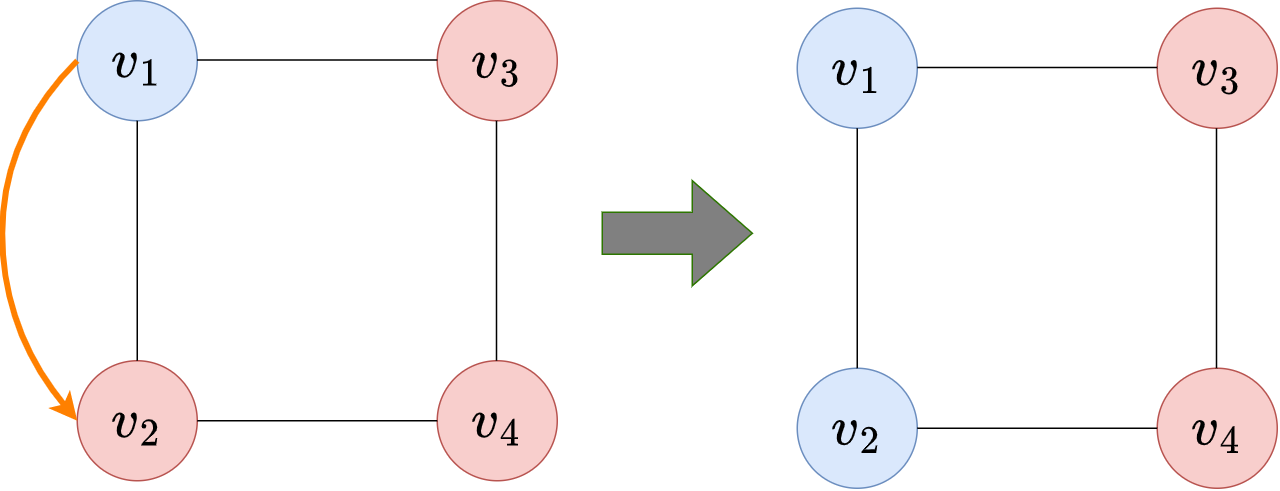
\includegraphics[scale=0.2]{img/shift-neighbor.png}
  \caption{シフト近傍}
  \label{shift-neighbor}
\end{figure}

\subsection{スワップ近傍}

スワップ近傍は,2つの部分グラフに含まれる頂点のラベルを交換する近傍操作である.
スワップ近傍の例として,図\ref{swap-neighbor}を用いて説明する.
先ほどと同様に,青色の頂点集合からなる部分グラフを$\mathcal{G}_1$,
赤色の頂点集合からなる部分グラフを$\mathcal{G}_2$とする.
$\mathcal{G}_1$には頂点$v_1$が含まれており,$v_1$は.
$\mathcal{G}_2$の頂点$v_3$と隣接している.
また,$\mathcal{G}_2$には頂点$v_4$が含まれており,$v_4$は.
$\mathcal{G}_1$の頂点$v_2$と隣接している.
スワップ近傍では,頂点$v_1$のラベル$x[v_1]$を
頂点$v_3$のラベル$x[v_3]$に代入し,
頂点$v_4$のラベル$x[v_4]$を
頂点$v_2$のラベル$x[v_2]$に代入する.
すると,$\mathcal{G}_1$と$\mathcal{G}_2$に含まれる頂点が
それぞれ一つずつ交換された近傍解ができる.
このように,2つの部分グラフ間で頂点を交換することで,
シフト近傍のみでは遷移できない近傍解が作られ,
解の精度が上がりやすくなる.

\begin{figure}[htbp]
  \centering
  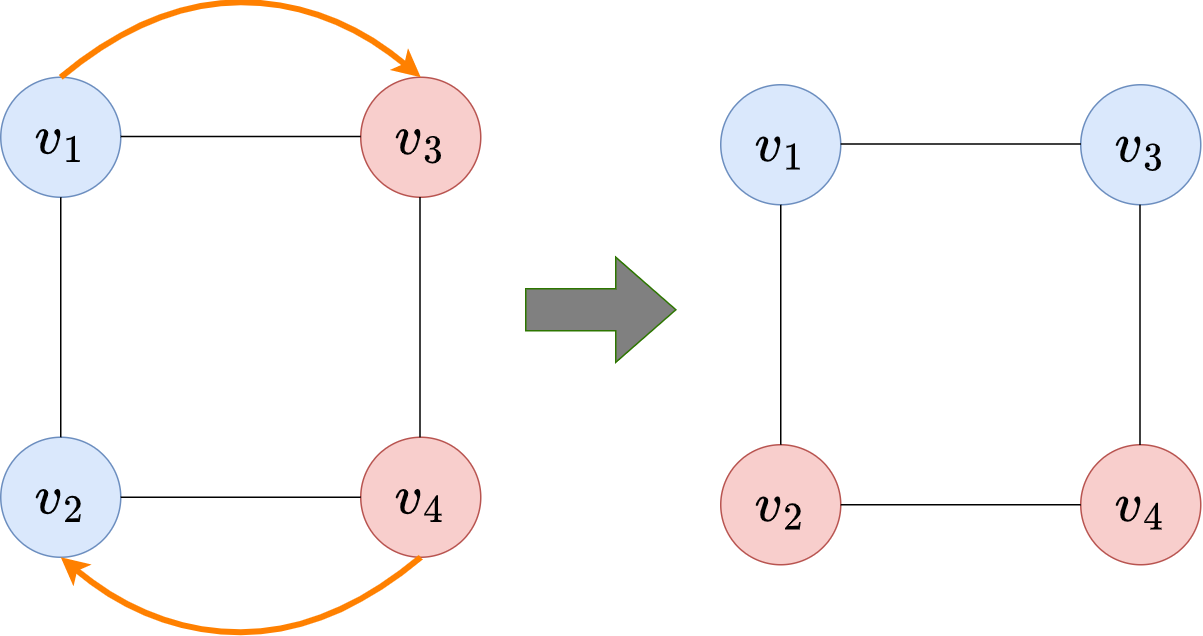
\includegraphics[scale=0.2]{img/swap-neighbor.png}
  \caption{スワップ近傍}
  \label{swap-neighbor}
\end{figure}

\subsection{2連鎖シフト近傍}

2連鎖シフト近傍とは,一つの部分グラフを主軸として,
2回のシフト近傍操作を同時に行うものである.
2連鎖シフト近傍の例として,図\ref{chain-neighbor}を用いて説明する.
青色の頂点集合からなる部分グラフを$\mathcal{G}_1$,
赤色の頂点集合からなる部分グラフを$\mathcal{G}_2$,
緑色の頂点集合からなる部分グラフを$\mathcal{G}_3$とする.
$\mathcal{G}_2$を主軸に置くと,$\mathcal{G}_1$に頂点$v_2$を渡すが,
$\mathcal{G}_3$から,頂点$v_6$を受け取る.
このようにある部分グラフが,頂点を1つ渡し,1つ受け取る操作を行うことで,
シフト近傍やスワップ近傍では得られなかった近傍解を作成することができる.

なお,一般的に連鎖シフトは,3回以上シフト近傍操作を行うものも存在するが,
選挙区割問題では必要性は低いと判断し,実装は行わなかった.

\begin{figure}[htbp]
  \centering
  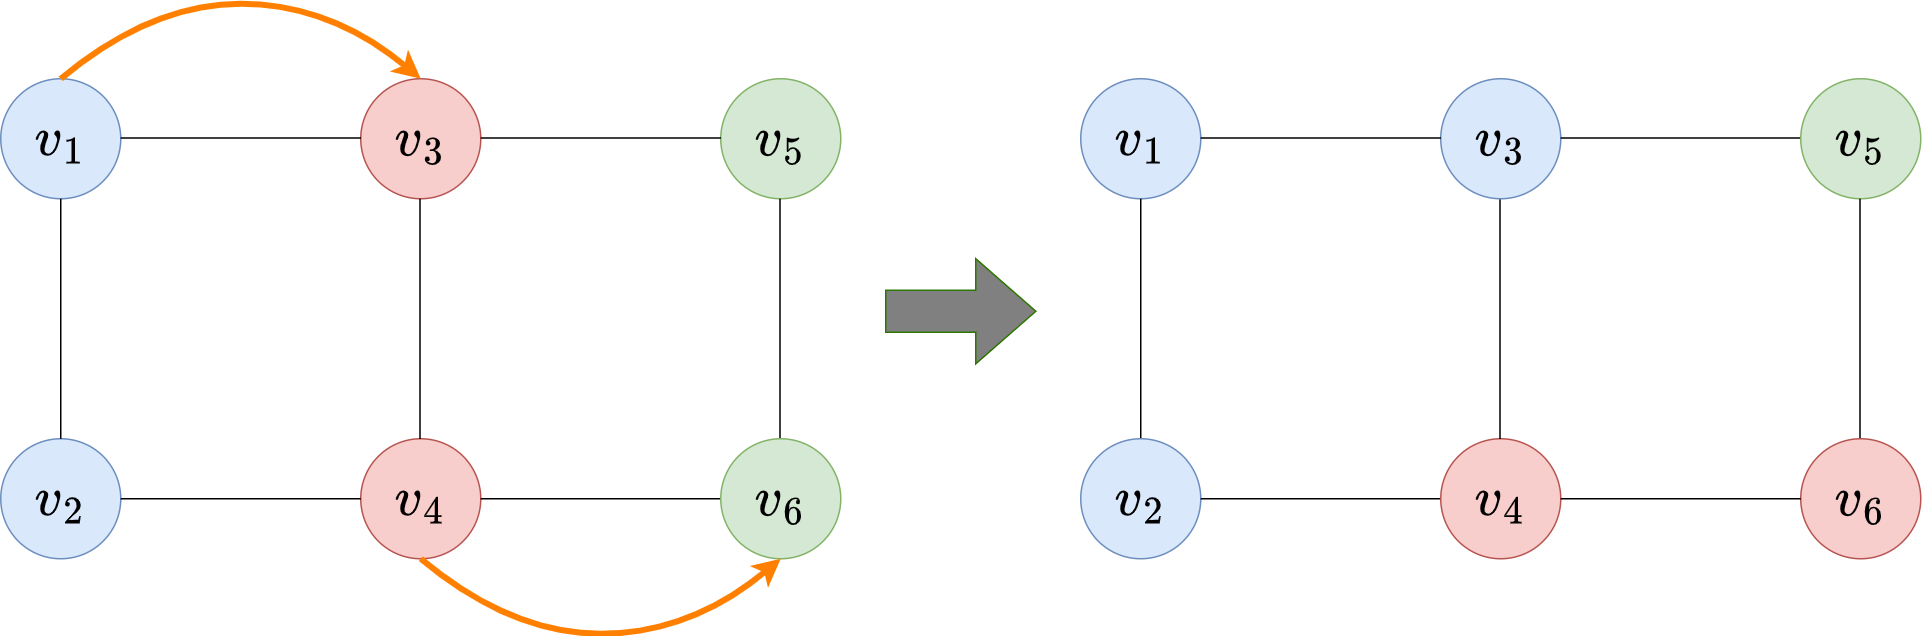
\includegraphics[scale=0.2]{img/chain-neighbor.png}
  \caption{2連鎖シフト近傍}
  \label{chain-neighbor}
\end{figure}

\section{焼きなまし法}

焼きなまし法とは,現在の解$x$から作られた近傍解$x'$が改善解なら移動し,
改悪解ならばスコアの値の変化量$\Delta=f(x')-f(x)$に応じた確率で
移動することで,質の低い局所最適解から脱出し,より良い解を探索する
手法である\cite{umetani}.
選挙区割問題での改善解は$\Delta \leq 0$,改悪解は$\Delta > 0$となる.
改悪解に遷移する確率は,温度と呼ばれるパラメータ$t$により
$e^{-\Delta/t}$と設定する.

焼きなまし法の手続きを以下にまとめる.
\begin{description}
  \item[Step 1:] 初期解$x$を生成する.暫定解$x^{\natural}=x$とする.
  初期温度$t_s$を設定し,$t=t_s$とする.
  \item[Step 2:] 3つの近傍操作をランダムに選択し,
  現在の解$x$から選んだ近傍操作で生成した近傍解を$x'$とする.
  \item[Step 3:] $x'$が問題の制約を満たしているか判定し,
  満たしていなければ\textbf{Step 2}に戻る.
  \item[Step 4:] $\Delta=f(x')-f(x)$とし,$\Delta \leq 0$ならば
  確率$1$,$\Delta > 0$ならば確率$e^{-\Delta/t}$で$x=x'$とする.
  \item[Step 5:] $f(x)<f(x^{\natural})$ならば$x^{\natural}=x$とする.
  \item[Step 6:] 終了条件を満たせば$x^{\natural}$を出力して終了.そうでなければ,
  温度$t$を更新して\textbf{Step 2}に戻る.
\end{description}

焼きなまし法を実装するには,初期温度,温度の更新方法,
アルゴリズムの終了条件などを定める必要がある.
初期温度$t_{s}$は,一回の遷移で動きうるスコア幅の最大値程度にしたいため,
考えられるスコアの最大値$-$最小値に近い値を設定する.
スコアの最小値は全てのケースで$1$を下回ることはない.
考えられるスコアの最大値は概算で求める.
まず,グラフの頂点重みを昇順にソートしたものを$w'_1,\ldots,w'_n$とおく.
部分グラフの最大重みは,連結であることを考慮しなければ
$\sum_{i=d}^n w'_i$,最小重みは$w'_1$であるから,
求めるスコアの最大値は,$(\sum_{i=d}^n w'_i)/w'_1$となる.
よって,初期温度は$$t_s=\frac{\sum_{i=d}^n w'_i}{w'_1}- 1$$と定める.
また,終了温度$t_e$は一回の遷移で動きうるスコア幅の最小値程度にしたい.
ただし,スワップ近傍で限りなく小さいスコア幅で遷移することもあるため,
今回は$t_e=0$とし,現在温度が終了温度に達した($t=t_e$)場合に
アルゴリズムは終了条件を満たしたと判定する.

温度の更新方法については,
制限時間$T_{limit}$,経過時間$T_{now}$を用いて,現在温度$t$を定義すると,
$$t=t_s - (t_s - t_e)\cdot \frac{T_{now}}{T_{limit}}$$
となる.$T_{limit}$は問題の規模に合わせて手動で調整する.

